\documentclass[supercite]{Experimental_Report}

\title{~~~~~~新生实践课~~~~~~}
\author{陈英睿}
\school{计算机科学与技术学院}
\classnum{创新2401}
\stunum{U202414898}
\instructor{范晔斌} 
\date{2024年11月28日}

\usepackage{algorithm, multirow}
\usepackage{algpseudocode}
\usepackage{amsmath}
\usepackage{amsthm}
\usepackage{framed}
\usepackage{mathtools}
\usepackage{subcaption}
\usepackage{xltxtra} 
\usepackage{bm}
\usepackage{tikz}
\usepackage{tikzscale}
\usepackage{pgfplots}
%\usepackage{enumerate}

\pgfplotsset{compat=1.16}

\newcommand{\cfig}[3]{
  \begin{figure}[htb]
    \centering
    \includegraphics[width=#2\textwidth]{images/#1.tikz}
    \caption{#3}
    \label{fig:#1}
  \end{figure}
}

\newcommand{\sfig}[3]{
  \begin{subfigure}[b]{#2\textwidth}
    \includegraphics[width=\textwidth]{images/#1.tikz}
    \caption{#3}
    \label{fig:#1}
  \end{subfigure}
}

\newcommand{\xfig}[3]{
  \begin{figure}[htb]
    \centering
    #3
    \caption{#2}
    \label{fig:#1}
  \end{figure}
}

\newcommand{\rfig}[1]{\autoref{fig:#1}}
\newcommand{\ralg}[1]{\autoref{alg:#1}}
\newcommand{\rthm}[1]{\autoref{thm:#1}}
\newcommand{\rlem}[1]{\autoref{lem:#1}}
\newcommand{\reqn}[1]{\autoref{eqn:#1}}
\newcommand{\rtbl}[1]{\autoref{tbl:#1}}

\algnewcommand\Null{\textsc{null }}
\algnewcommand\algorithmicinput{\textbf{Input:}}
\algnewcommand\Input{\item[\algorithmicinput]}
\algnewcommand\algorithmicoutput{\textbf{Output:}}
\algnewcommand\Output{\item[\algorithmicoutput]}
\algnewcommand\algorithmicbreak{\textbf{break}}
\algnewcommand\Break{\algorithmicbreak}
\algnewcommand\algorithmiccontinue{\textbf{continue}}
\algnewcommand\Continue{\algorithmiccontinue}
\algnewcommand{\LeftCom}[1]{\State $\triangleright$ #1}

\newtheorem{thm}{定理}[section]
\newtheorem{lem}{引理}[section]

\colorlet{shadecolor}{black!15}

\theoremstyle{definition}
\newtheorem{alg}{算法}[section]

\def\thmautorefname~#1\null{定理~#1~\null}
\def\lemautorefname~#1\null{引理~#1~\null}
\def\algautorefname~#1\null{算法~#1~\null}

\begin{document}

\maketitle

\clearpage

\pagenumbering{Roman}

\tableofcontents[level=2]
\clearpage

\pagenumbering{arabic}

\section{网页整体框架}
我总共编写了5个页面,首先我在主页面中确定了内容的主题:我最喜欢的人物——宋徽宗,并将其余4个页面用来介绍人物,这4个页面分别从人物生平,书法成就,绘画作品以及园林造诣展开。
\begin{figure}[H]
  \centering
  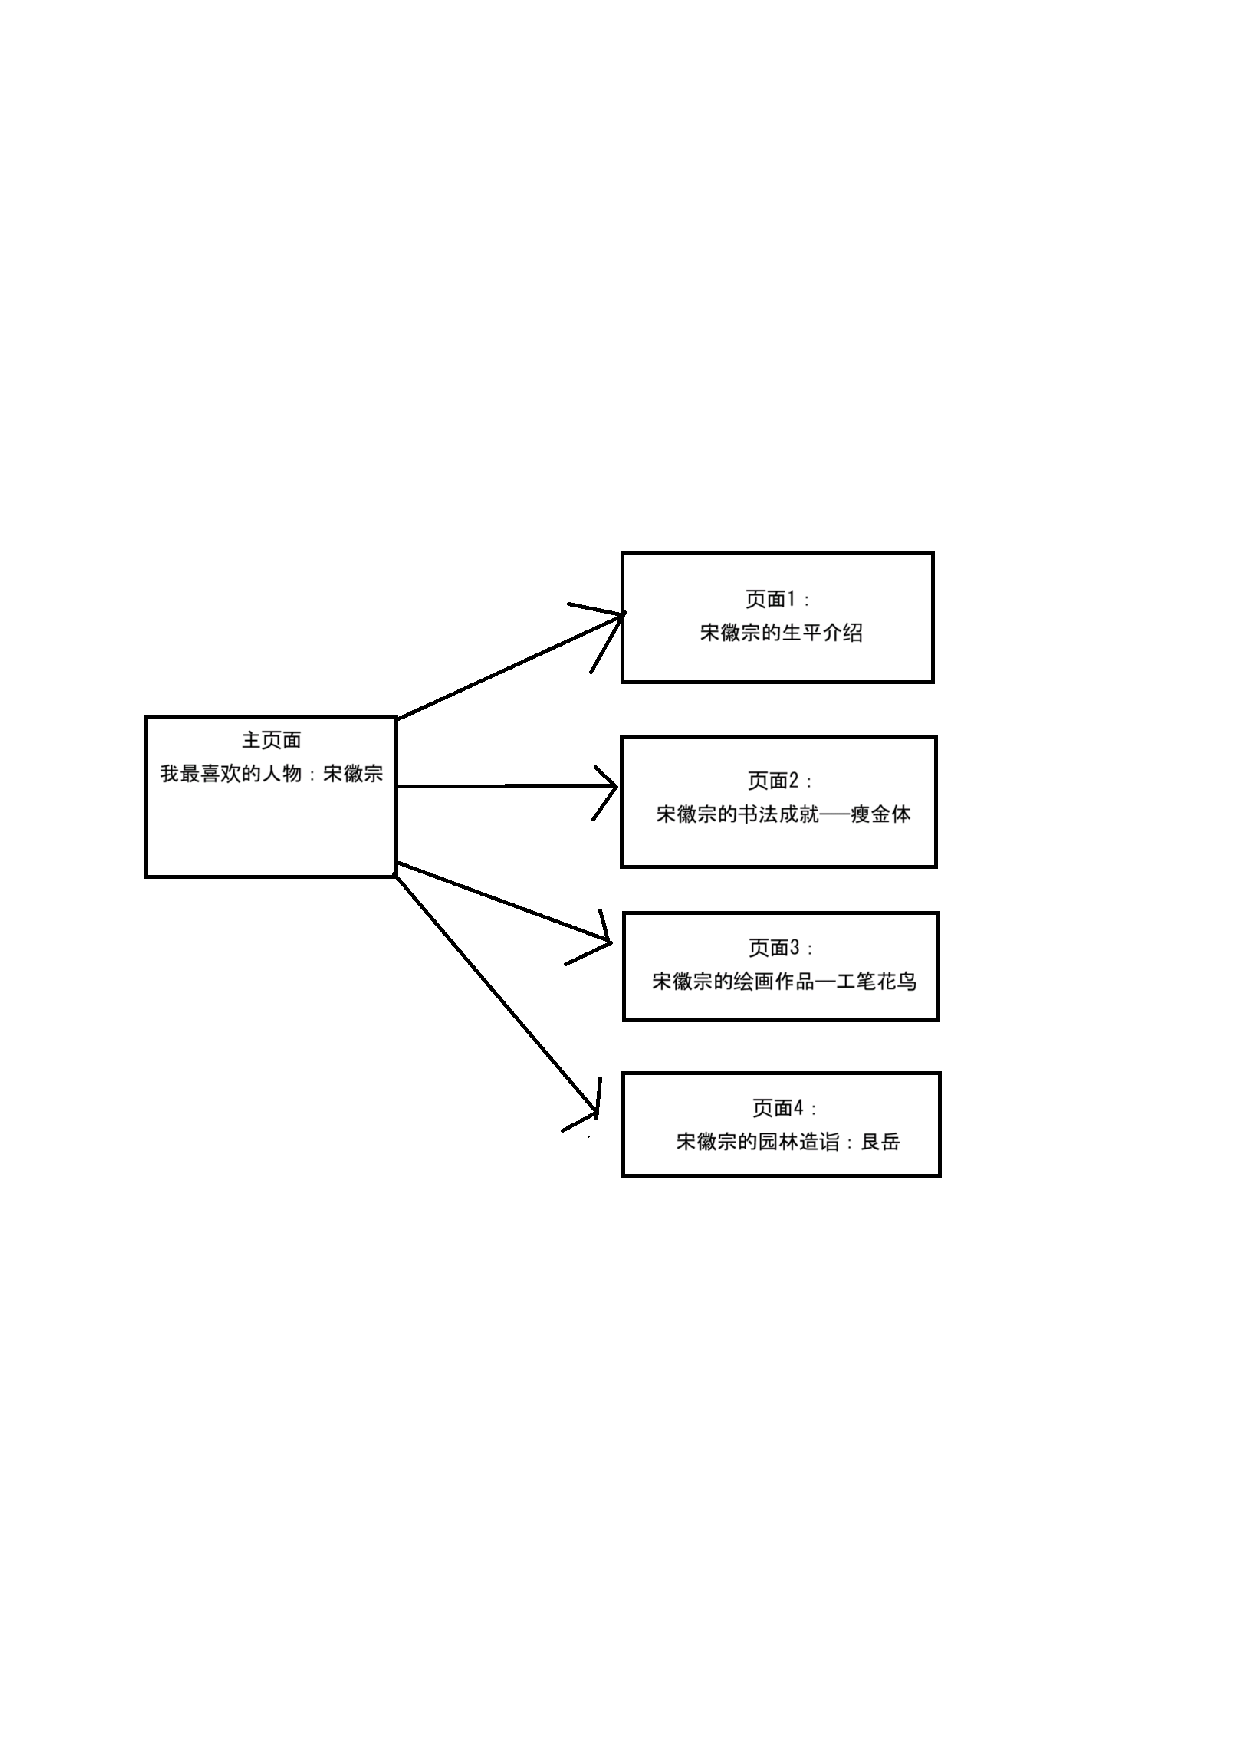
\includegraphics[width=0.75\linewidth]{./images/页面框架.pdf}
  \caption{网页整体框架}
  \label{fig:enter-label}
\end{figure}

\newpage

\section{主页设计}
在主页中,我首先给出了我的id:ruoshui,并用黄色字体,加粗与居中修饰。在下面我直接展示出了我本次网页的主题:我最喜欢的人物:宋徽宗,同时为了启到强调作用,我也将宋徽宗3字做了黄色字体处理。为了主页的美观,我上网搜寻了一张画面宏大且精美的图片,该图展示了一幅美丽的山水画,山峰被白雪覆盖,湖水清澈,树木在秋天的阳光下呈现出金黄色的色彩,整个画面给人一种宁静而祥和的感觉,故我将该图设置为主页的背景。
\par 然后我分别设置了4个按钮于文字的下方作为导航,分别前往我的其余4个页面——生平简介,书法成就,绘画作品,园林造诣。
\begin{figure}[H]
    \centering
    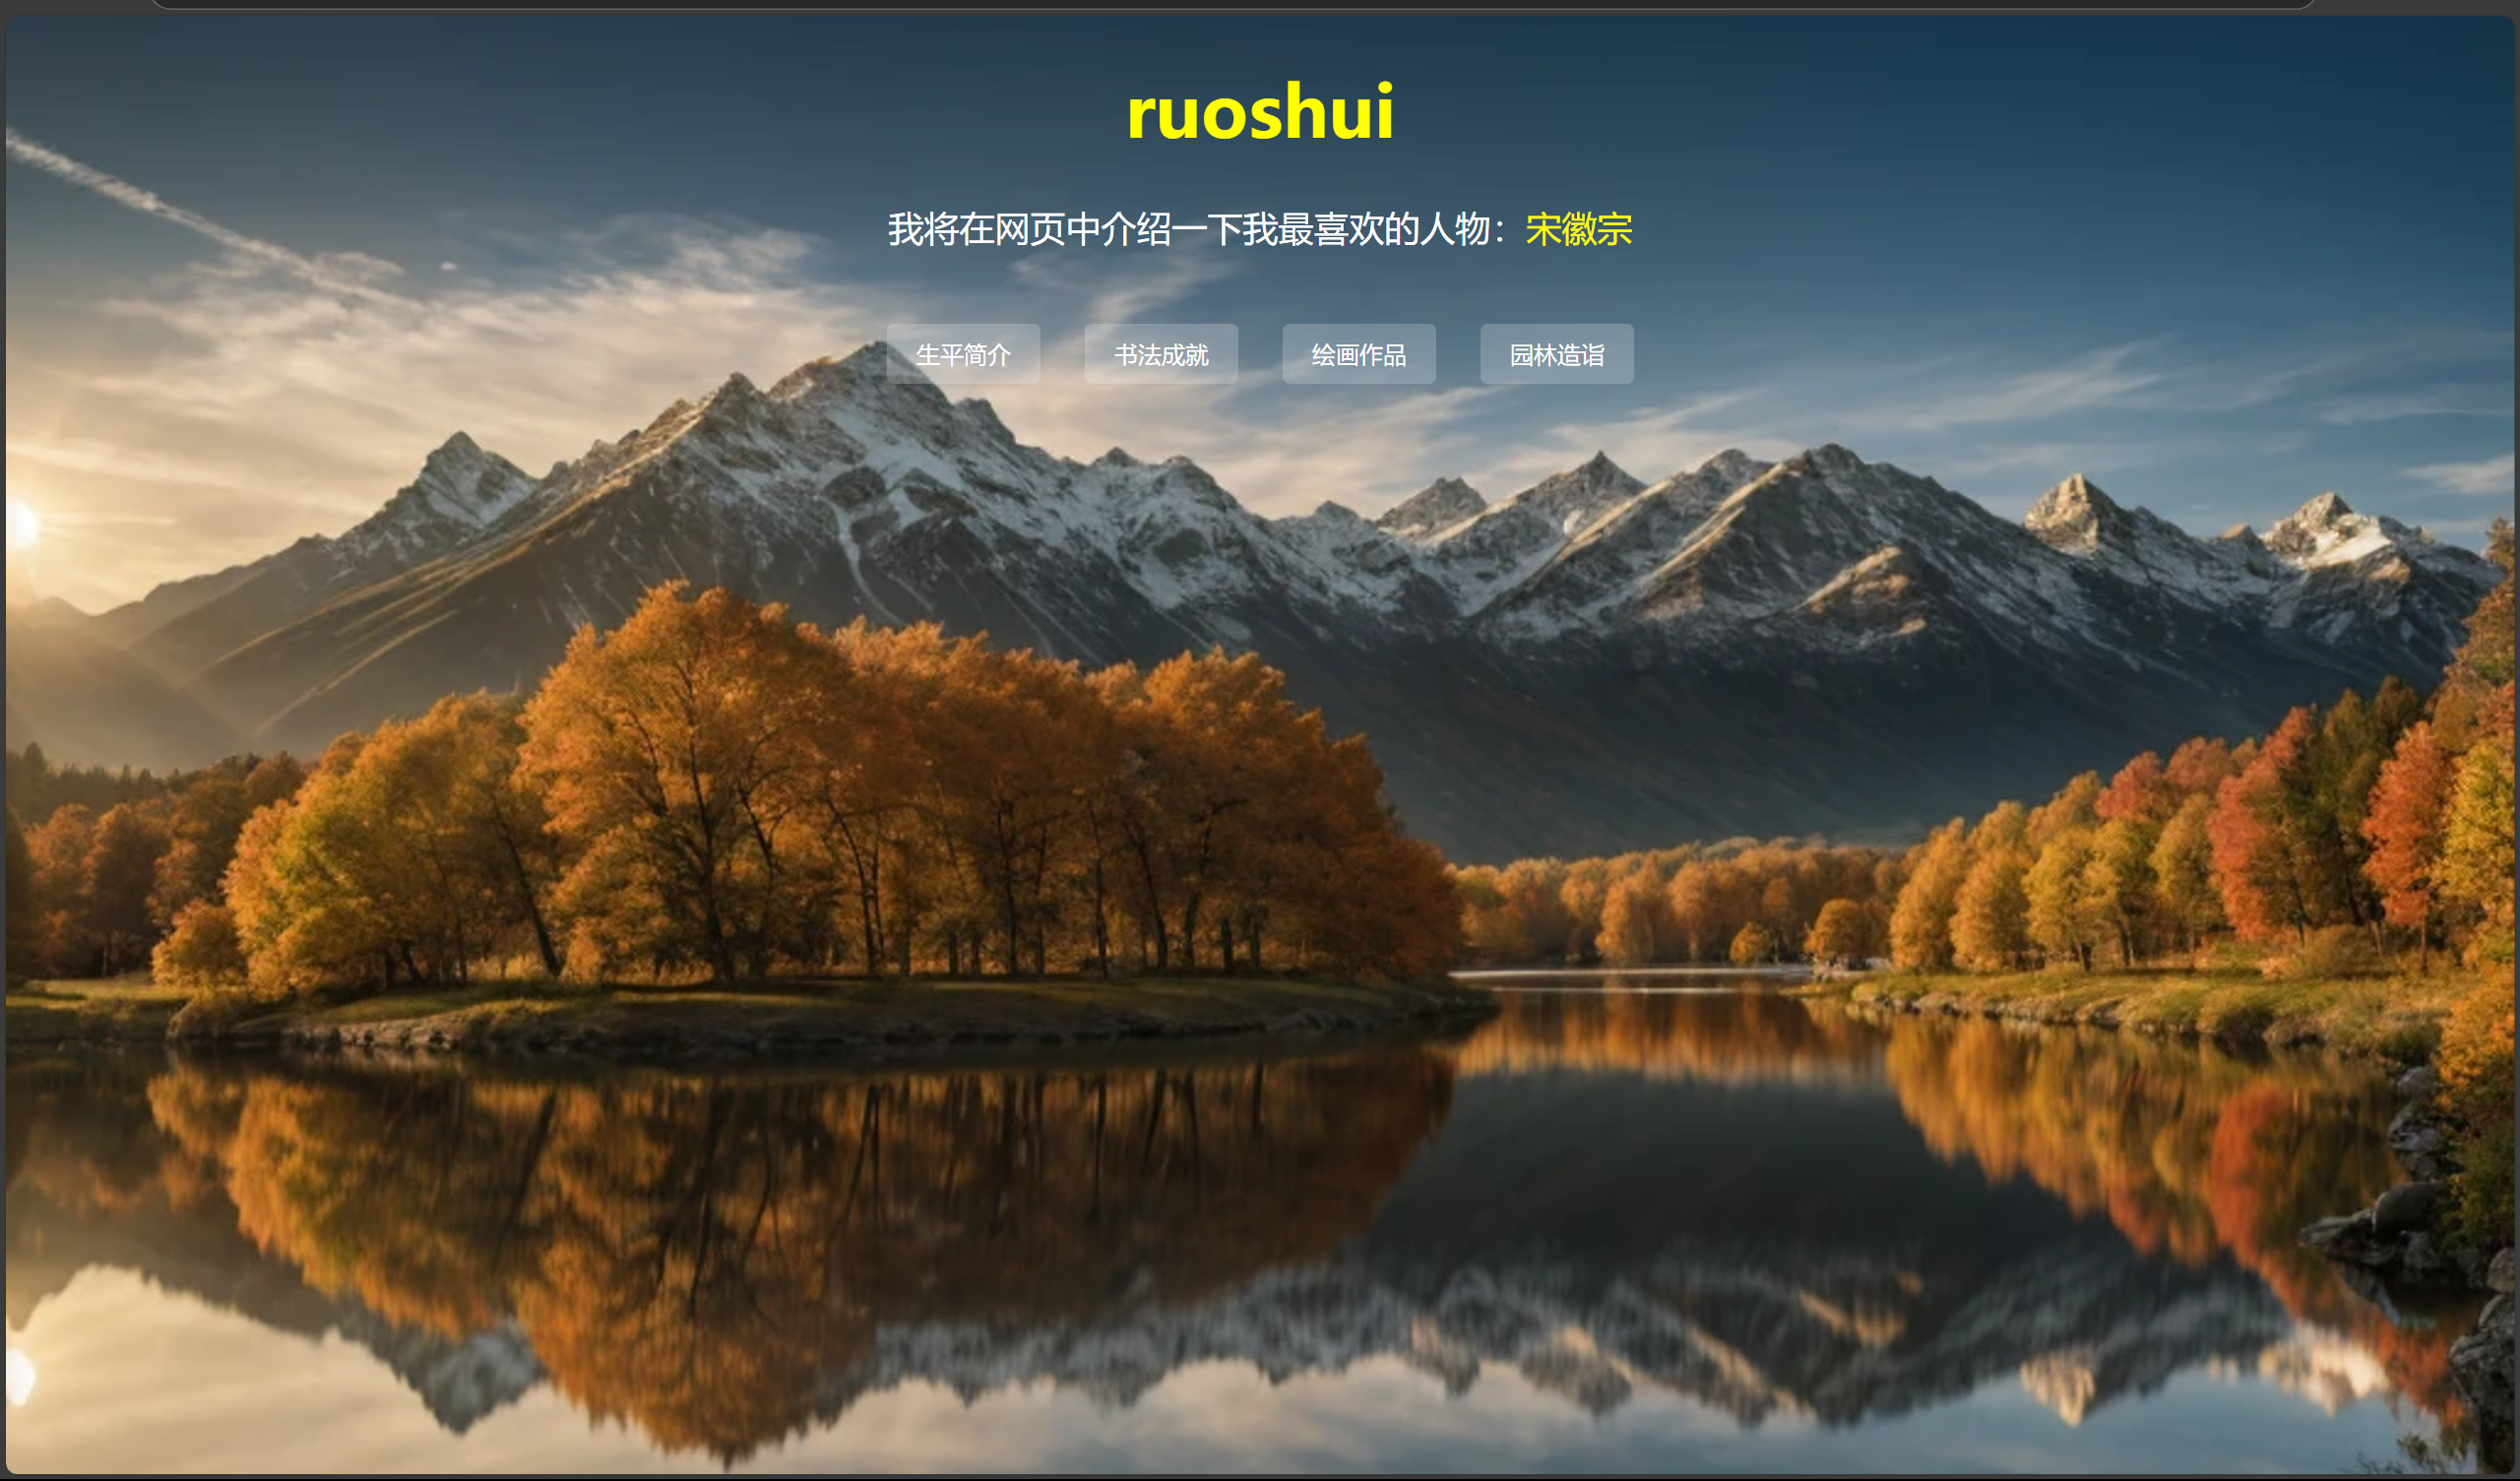
\includegraphics[width=1\linewidth]{./images/主页面.png}
    \caption{主页背景}
    \label{fig:enter-label}
\end{figure}

\newpage

\section{分页面设计}

我将在一下介绍各个分页面的内容与设计思路,并展示我的各个分页面。

\subsection{人物生平}
在设计人物生平的网页时,首先为了用户能够一眼把握网页的主题,我在网页的头部加上了”宋徽宗生平简介“,以便读者更好的了解内容。同时为了各个网页的连通,我在头部也添加了四个超链接,以便用户可以通过各个链接访问到不同的网页。为了更好的突出生平简介中的内容,我将”瘦金体“字体处理为粉色,将宋徽宗的作品如:《芙蓉锦鸡图》《祥龙石图》设置为蓝色,以提升用户的体验。
\begin{figure}[H]
    \centering
    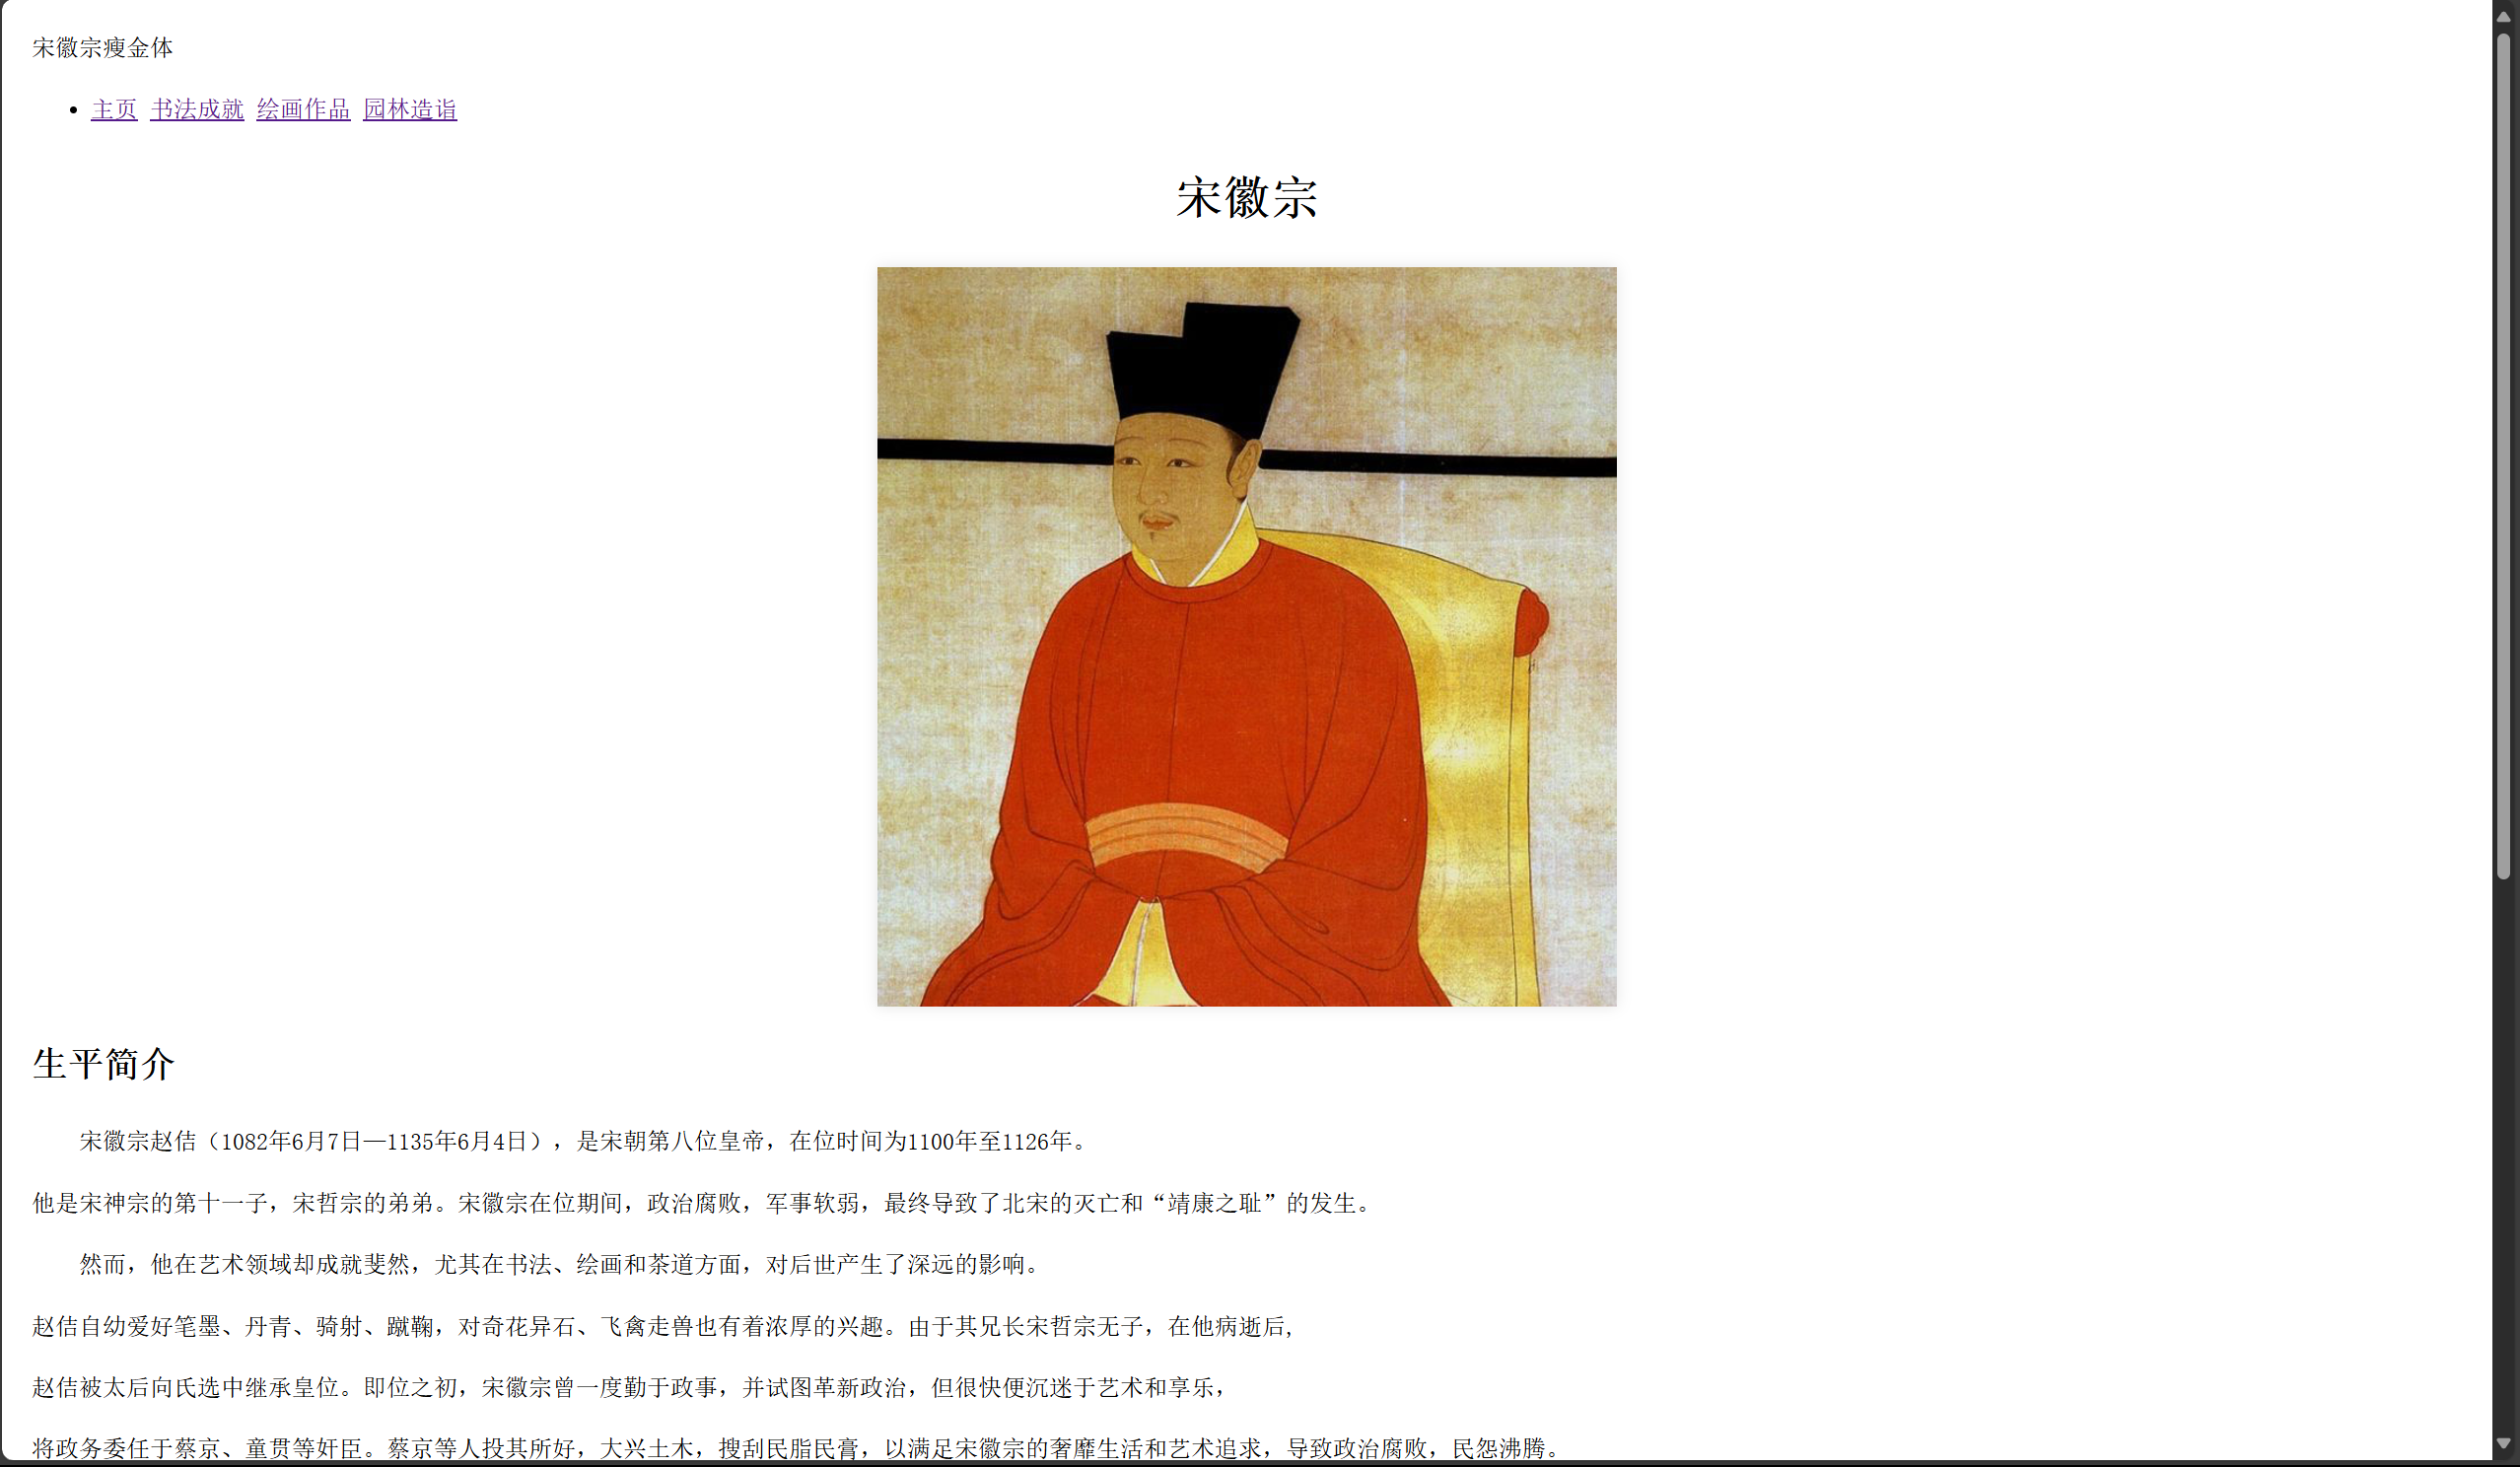
\includegraphics[width=1\linewidth]{./images/人物生平.png}
    \caption{人物生平}
    \label{fig:enter-label}
\end{figure}
\par 在网页的正中央,我添加了一张宋徽宗图片,并在上方加粗居中标注:宋徽宗。接着我便开始了宋徽宗的生平简介,包括他的身份地位,出生时间,在位时间。以下为我在网页中摘取的部分内容。
\begin{abstract}
    宋徽宗赵佶(1082年6月7日—1135年6月4日),是宋朝第八位皇帝,在位时间为1100年至1126年。
他是宋神宗的第十一子,宋哲宗的弟弟。宋徽宗在位期间,政治腐败,军事软弱,最终导致了北宋的灭亡和“靖康之耻”的发生。然而,他在艺术领域却成就斐然,尤其在书法、绘画和茶道方面,对后世产生了深远的影响。赵佶自幼爱好笔墨、丹青、骑射、蹴鞠,对奇花异石、飞禽走兽也有着浓厚的兴趣。由于其兄长宋哲宗无子,在他病逝后,
赵佶被太后向氏选中继承皇位。即位之初,宋徽宗曾一度勤于政事,并试图革新政治,但很快便沉迷于艺术和享乐,
将政务委任于蔡京、童贯等奸臣。蔡京等人投其所好,大兴土木,搜刮民脂民膏,以满足宋徽宗的奢靡生活和艺术追求,导致政治腐败,民怨沸腾。
\par 在艺术方面,宋徽宗极具天赋,且勤奋钻研。他独创的“瘦金体”书法,以其独特的瘦劲、
挺拔和锋利,成为书法史上一颗璀璨的明珠。这种字体笔画细瘦,但骨力遒劲,体现了宋徽宗独特的审美追求。
在绘画方面,宋徽宗尤擅花鸟画,他注重写生,观察细致入微,笔下的花鸟栩栩如生,设色艳丽,极具艺术感染力。他创立了皇家画院——翰林图画院,
并亲自指导画家创作,对宋代绘画艺术的发展起到了重要的推动作用。他的一些传世名作,如《芙蓉锦鸡图》《祥龙石图》等,至今仍被视为珍贵的艺术瑰宝。
此外,宋徽宗还精通茶道,著有《大观茶论》,对宋代茶文化的发展也做出了贡献。然而,宋徽宗的艺术造诣并不能掩盖他在政治上的昏庸无能。
\par 在军事上,他指挥失误,导致对辽战争和对金战争的失败,最终使得金兵攻破汴京,北宋灭亡。他重用奸臣,不理朝政,导致政治腐败,社会矛盾激化
1127年,宋徽宗与儿子宋钦宗一起被金人俘虏北上,史称“靖康之耻”,北宋的繁华景象也随之烟消云散。被俘后,宋徽宗被金人囚禁于五国城(今黑龙江省依兰县),
度过了屈辱的八年囚徒生活。1135年,宋徽宗病逝于五国城,终年54岁,他的命运也成为了后世帝王的警示。
\par 宋徽宗的一生充满了矛盾和争议,他在艺术上的辉
煌成就与政治上的昏庸无能形成了鲜明的对比。他虽然创造了极高的艺术价值,却也为北宋的灭亡承担了不可推卸的责任。他的故事也警示后人,治国理政并非儿戏,沉迷享乐和玩物丧志最终只会导致国家的衰败和人民的苦难。
\end{abstract}


\subsection{书法成就}

在书法成就页面中,同人物生平,我在头部加上了”宋徽宗瘦金体“,并设置了4个超链接。在书法页面中,我在网页设置了主图与4个次图,主图我引用了岳飞的《满江红》用来引入,由于我本身也是一名书法爱好者,故在主图的右边加上了我对书法的看法与理解。在次图中,我分别添加了宋徽宗的《夏日诗贴》临摹,《夏日诗帖》原帖,《牡丹诗帖》原帖,《牡丹诗帖》临摹这4张图片,为了用一个更好的方式容纳这4张图片。我将每张图片的width设为25,padding为15px,与box-sizing: border-box。在每张图片的下方,我将图片的标题加粗并居中显示,在标题的下方添加说明文字。我选取了最具有代表性的宋徽宗两张帖照片,为了使用户更好的了解宋徽宗,突出我本次网页的主题。

\begin{figure}[H]
    \centering
    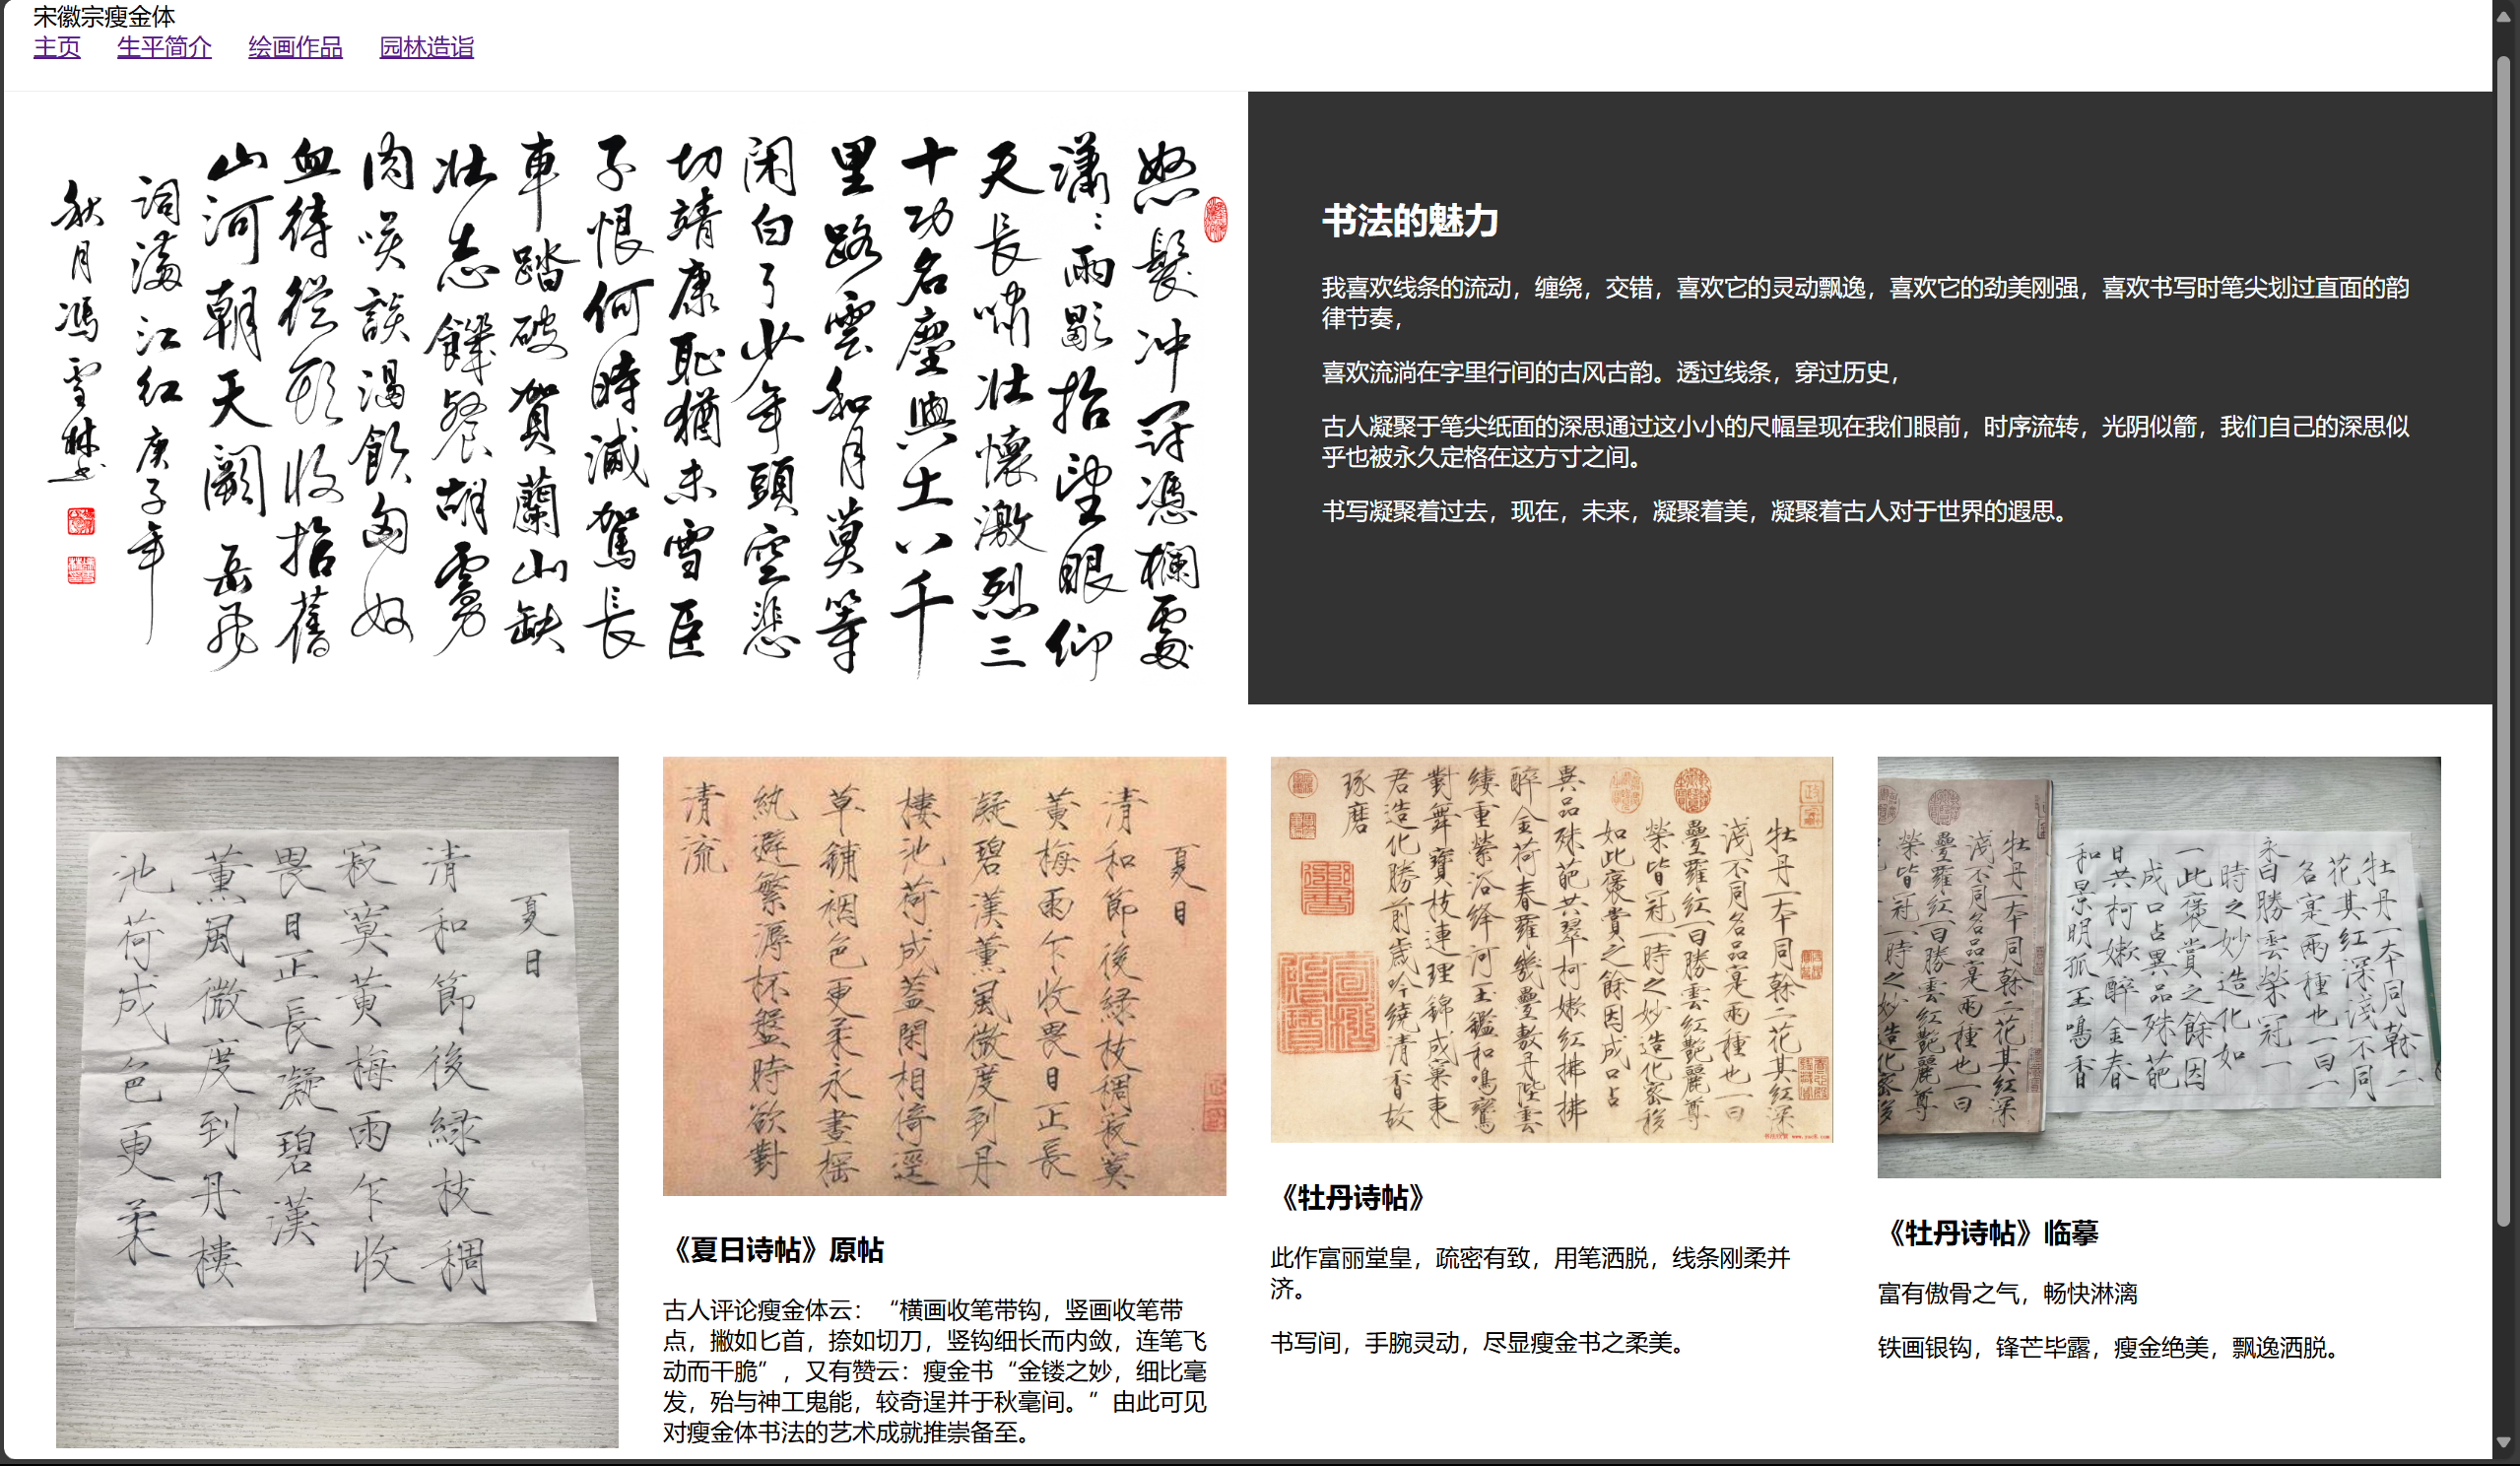
\includegraphics[width=1\linewidth]{./images/书法成就.png}
    \caption{书法成就}
    \label{fig:enter-label}
\end{figure}

\subsection{绘画作品}
\par 艺术作品布局:我选择了将所有作品按照名字排列的方式展示,这样用户可以清晰地看到每一幅作品的标题,方便他们快速找到感兴趣的作品。同时,这种布局方式也使得整个网页看起来整洁有序。
\par 作品展示:每个作品都有详细的介绍文字,这有助于用户了解每一幅作品的背景和特点。我特别注意了字体的大小和颜色,确保文字清晰易读,不会影响用户的阅读体验。
\par 导航设计:网页的顶部和底部都有明确的导航栏,用户可以通过这些导航栏快速跳转到不同的部分。
\par 视觉效果:我使用了深灰色的背景色,这样可以突出艺术作品的颜色和细节。同时,我还在网页中添加了一些装饰元素,如边框和表格,使整个网页看起来更加美观。
\par 我将最具有代表性的宋徽宗的工笔花鸟画展示更用户,旨在使用户对宋徽宗的绘画成就有一个更清晰的认识,完成我的网页的目的。
\begin{figure}
    \centering
    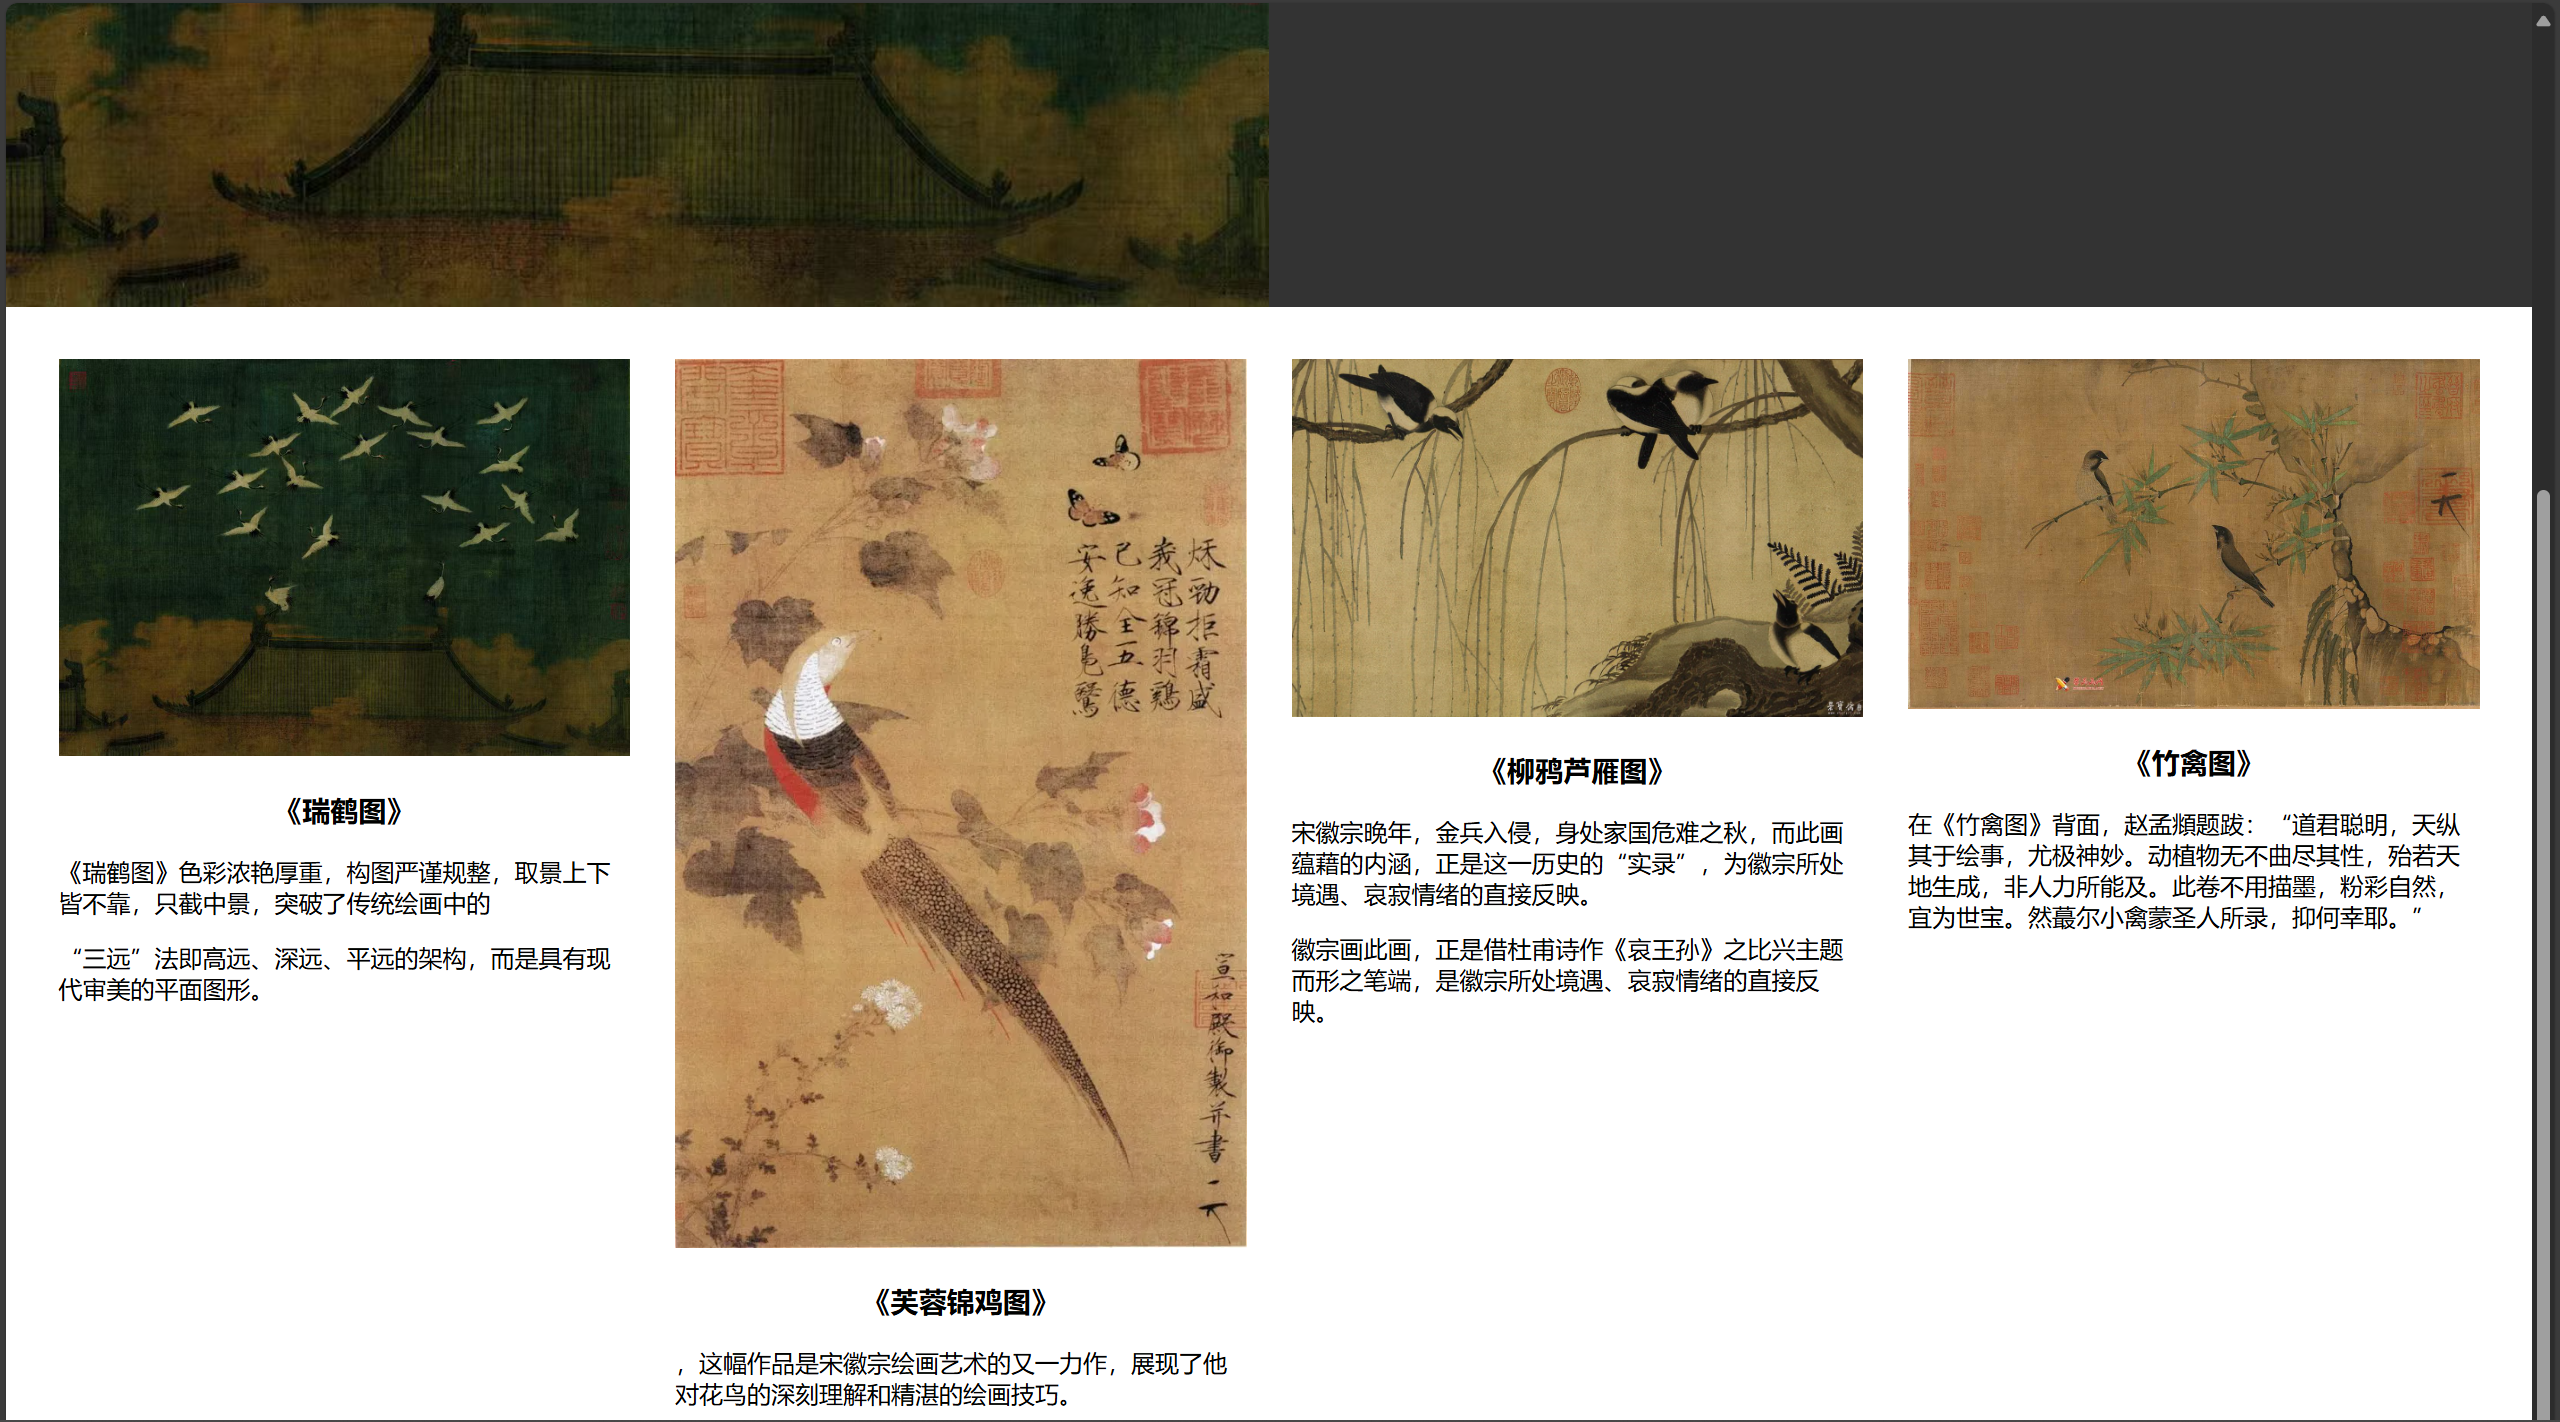
\includegraphics[width=1\linewidth]{./images/绘画作品.png}
    \caption{绘画作品}
    \label{fig:enter-label}
\end{figure}
\subsection{园林造诣}

在园林造诣页面中,,我首先明确了核心内容的框架,即围绕“宋徽宗园林造诣”这一主题,划分了几个关键模块:引言、宋徽宗的园林风格、著名园林、影响与遗产。这样的分块设计是为了确保用户能迅速抓住主要信息,而不至于在繁杂的内容中迷失方向。
\par 引言部分:我将宋徽宗的基本信息和他在园林艺术史上的地位作为开篇,既是对主题的总体概括,也为用户提供背景知识,帮助他们理解后续内容。
\par 园林风格:这是全文的核心部分,我进一步细分为“自然融合、精致设计、文化内涵”三个小点,通过简洁的条列式结构突出宋徽宗园林艺术的特点,避免大段文字堆砌导致的阅读疲劳。
著名园林:这里选择了两个具有代表性的园林实例“花石纲”和“东苑”,通过具体的案例讲述宋徽宗园林设计的实践成果,让内容更具说服力和吸引力。
\par 影响与遗产:最后总结宋徽宗园林艺术的历史意义和传承价值,升华主题,为网页内容画上一个完整的句号。
这样的内容结构设计注重层次分明和逻辑清晰,让用户能按顺序逐步深入了解主题。
宋徽宗是一个充满艺术审美的人物,因此在视觉设计上,我希望能体现出宋代的文化氛围,同时保持现代网页设计的简约风格。
\par 留白设计:为了避免信息过载,我在每个模块之间留出了足够的空白区域,这不仅让页面看起来更干净,也给用户提供了视觉上的缓冲。
\begin{figure}[H]
    \centering
    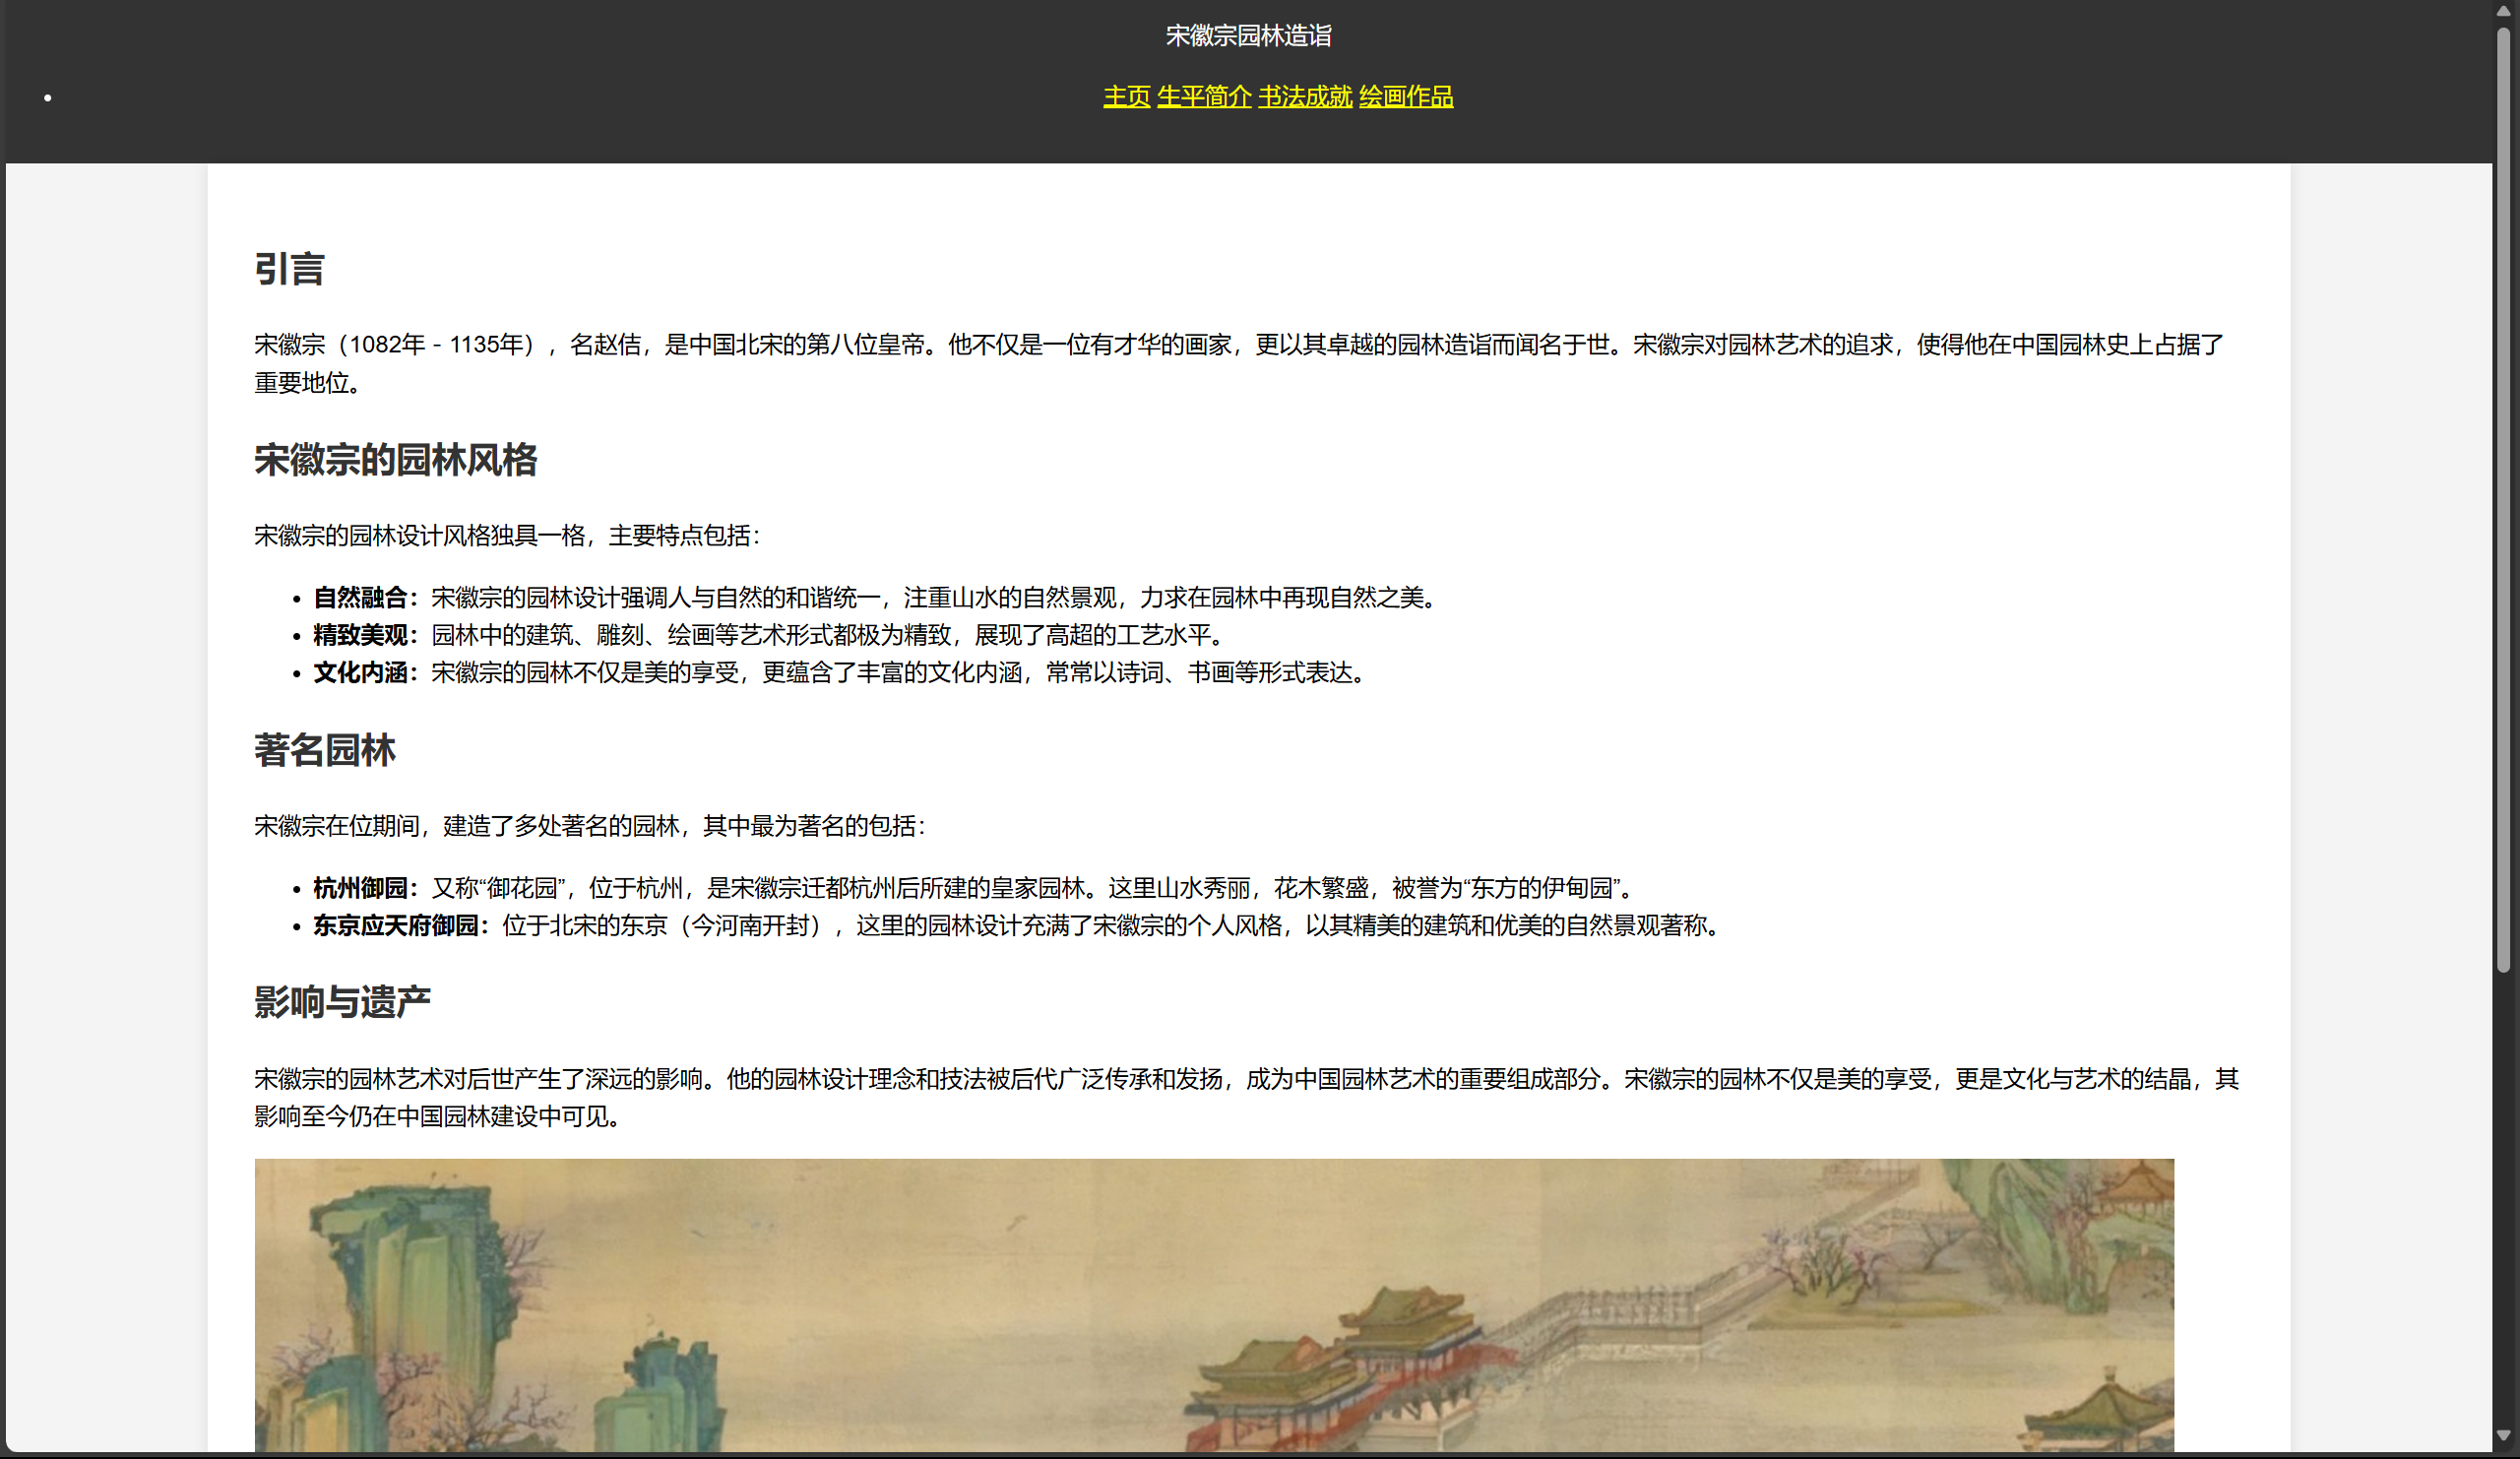
\includegraphics[width=1\linewidth]{./images/园林造诣.png}
    \caption{园林造诣}
    \label{fig:enter-label}
\end{figure}

\section{网页设计小结}

在主页面的设计和实现过程中,我遇到的最大的困难就是制作按钮的效果,按钮的样式需要精确调整,以确保美观和一致性,同时要确保背景图片的正确路径和尺寸设置,以便在不同设备和屏幕尺寸上都能正确显示。在生平简介网页中,较为困难的时做好页面的布局以及完成相关字体的颜色改变,在书法成就网页中,最大的困难在于排版好4张此图的位置,以便有更好的用户体验。
\par 而在实现网页的过程中,我遇到的最大的困难便是图片的相对路径处理,由于我最开始并没有创建文件夹,而是将所有的文件有图片都放在大的文件夹下面,并且我的图片路径使用的时相对路径。而我后面再创建了image和web文件夹,再次打开网页时所有的图片都消失了,最开始我难以发现问题的所在,直到最后重新添加了每一张图片的新的路径,这个问题才得以解决。

\newpage

\section{课程的收获和建议}


\subsection{计算机基础知识}
通过系统地学习计算机基础知识专题,我收获颇丰,主要体现在以下几个方面:

\par 1.构建了扎实的理论基础:
理解了计算机的组成原理: 深入了解了计算机硬件的各个组成部分,如CPU、内存、存储设备、输入/输出设备等,以及它们之间的相互作用方式。这让我对计算机的工作原理有了更清晰的认识,不再仅仅停留在表面操作层面。
\par 2.掌握了数据表示与存储: 学习了二进制、八进制、十六进制等不同的数制,以及数据在计算机内部的表示方法,如整数、浮点数、字符等的编码方式。这让我能够更好地理解数据处理的本质,为后续的编程学习打下了坚实的基础。
\par 3.了解了操作系统原理: 学习了操作系统的基本概念、功能和分类,深入了解了进程管理、内存管理、文件系统等核心机制。这让我对计算机的运行方式有了更全面的理解,能够更好地利用操作系统提供的功能。
\par 4.熟悉了计算机网络基础: 学习了网络协议、网络拓扑结构、IP地址、等基本概念,了解了数据在网络中传输的原理。这让我对互联网的工作方式有了更深入的认识,为后续的网络编程学习奠定了基础。
\par 5.提升了问题分析与解决能力: 通过学习计算机基础知识,我能够更加系统地分析和解决计算机相关的问题。例如,当遇到电脑运行缓慢的问题时,我可以从多个方面进行排查,找到问题的根源并采取相应的措施。
\par 建议:可以适当增加git内容的学习时间和学习内容,git是一个十分有力的开发工具,在实际的开发过程中起的作用巨大,适当的深入学习git对以后的帮助极大。

\subsection{文档撰写工具LaTeX}
通过学习文档撰写工具LaTeX专题,我有以下收获:


\par 1.掌握了 LaTeX 的基本语法和结构: 能够使用 LaTeX 编写各种类型的文档,包括文章、报告、论文等。
\par 2.学习了 LaTeX 的常用宏包和命令: 能够使用各种宏包扩展 LaTeX 的功能,例如插入图片、表格、公式等。
\par 3.了解了 LaTeX 的文档编译流程: 能够使用 LaTeX 编辑器和编译器生成 PDF 文档。
\par 4.提高了文档排版的美观度和专业度: LaTeX 生成的文档格式规范、排版精美,更符合学术论文的规范要求。


\par 建议:适当增加“数学公式排版”的讲授内容和时间: 数学公式排版是 LaTeX 的核心功能之一,对于理工科专业的学生来说尤为重要。可以增加一些关于复杂数学公式排版的技巧和案例分析,例如,多行公式的对齐、大型运算符的使用、特殊符号的输入等,并适当增加练习环节,使我们学生通过实践加深理解。


\subsection{编程工具Python}
通过学习编程工具Python,我有以下收获:
\par 1.掌握了 Python 的基本语法和数据结构: 能够编写简单的 Python 程序,并使用列表、字典、元组等数据结构存储和处理数据。
\par 2.掌握了 Python 的函数和模块: 学习了如何定义和调用函数,以及如何使用模块来组织和复用代码,能够编写结构清晰、可维护的程序.
\par 3.掌握了 Python 的控制结构:学习了 Python 的条件语句(if-else)、循环语句(for、while)和异常处理机制(try-except),能够编写具有逻辑判断和流程控制的程序。提高了逻辑思维和问题解决能力: 学习编程需要逻辑思维和分析问题的能力,这提高了我的综合素质。



\par 建议:加强“Python 常用库的使用”的实践操作: Python 拥有丰富的第三方库,可以扩展 Python 的功能。可以增加一些实践操作环节,让同学们掌握如何使用常用的 Python 库。
。

\subsection{图像设计软件Photoshop}
通过学习图像设计软件Photoshop,我有以下收获:
\par 1.掌握了专业的图像处理技能:学习 Photoshop 之前,我对图像处理的认知仅限于简单的裁剪、调整亮度和对比度等。通过学习,我掌握了图层、蒙版、通道、滤镜、色彩调整、图像修复、文字设计等一系列专业技能,能够对图像进行精细化的处理和编辑。
\par 2.提升了审美能力和创意表达能力:Photoshop不仅仅是一款工具,更是一个创意表达的平台。通过学习,我逐渐培养了对色彩、构图、光影等视觉元素的敏感度,提升了审美能力。同时,我也学会了如何将自己的创意想法通过 Photoshop 付诸实践,创作出具有视觉冲击力和艺术感染力的作品。
\par 3.通过不断练习和实践,我的创意思维和设计能力得到了显著提升,能够更好地将设计理念转化为实际作品。

\par 建议:增加实用案例的教学:目前的课程中可能更多地集中在基础工具的讲解上,建议增加更多实际案例的教学,让学生能够看到这些工具在真实项目中的应用,增强学习的实用性和趣味性。

\subsection{版本管理软件Git}
通过学习版本管理软件Git,我有以下收获:

\par 1.理解了 Git 的工作原理: 学习了 Git 的版本控制思想,理解了仓库、提交、分支、合并等核心概念,对 Git 的工作流程有了清晰的认识。
\par 2.掌握了 Git 的基本命令: 能够熟练使用 Git 的常用命令,例如 init、add、commit、status、log、branch、merge、pull、push 等,能够完成代码的版本控制、提交、分支管理和合并等基本操作。
\par 3.能够进行代码版本管理: 学习了如何使用 Git 进行代码版本管理,能够回溯历史版本,查看代码修改记录,恢复误操作的代码,保证代码的安全性。
\par 4.了解了 Git 的应用场景: 了解了 Git 在软件开发、文档管理、网站部署等领域的应用,认识到 Git 的广泛应用价值。

\par 建议:分支管理和合并策略部分可以适当增加讲授内容和时间: 分支管理和合并策略是 Git 的核心功能,掌握它们能够提高团队协作效率,避免代码冲突。可以增加一些实际案例的分析和练习,例如如何创建和管理分支,如何解决合并冲突等。

\subsection{网页制作Dreamweaver}
通过学习网页制作Dreamweaver,我有以下收获:
\par 1.基本操作熟练掌握:通过老师的讲解和实践操作,我对Dreamweaver的基本功能有了深入的了解,比如如何创建和管理网页、使用CSS进行样式设计、插入图片和链接等。
\par 2.HTML和CSS的理解加深:虽然Dreamweaver提供了图形化界面,但是在实际操作中,还是需要对HTML和CSS有一定的了解。通过课程的学习,我对这些基础语言的理解得到了进一步的巩固和扩展,尤其是在代码视图中进行手动调整时,感觉对编程逻辑更加熟悉了。
\par 3.实践能力提升:通过多个实际项目的练习,比如制作个人主页、公司简介页面等,我增强了动手能力,也学会了如何将所学知识应用到实际网页制作中。每当完成一个网页时,看到自己的设计效果,成就感十足。

\par 建议:基础操作部分可适当减少:在Dreamweaver的初步操作部分,内容相对较为简单,比如如何新建文件、插入图片和文字等。这些内容可以适当压缩讲授时间,尤其是对于有一定计算机基础的同学来说,基础操作可以通过自学或课后练习掌握。
\nocite{*} %% 作用是不对文献进行引用,但可以生成文献列表
%\bibliographystyle{HustGraduPaper}
%\bibliography{HustGraduPaper}
\end{document}
